\section{Convolution-Augmented Attention: Conformer and Fast Conformer}
\label{sec:annex-conformer}

\subsection{Executive Summary}

The Conformer block \citep{Gulati2020} is the toolkit's convolution-augmented sequence mixer, exposed as \texttt{conformer}. It keeps the global receptive field of scaled dot-product attention and adds a depthwise-convolution branch that models local, narrow-band structure---the inductive bias speech recognition needs and the one plain self-attention lacks. The block sandwiches multi-head self-attention (MHSA) with relative sinusoidal positional encodings between two Macaron-style half-step feed-forward layers \citep{Lu2019}, and inserts the convolution module between the attention and the second FFN. In the reference recipe it reaches $1.9\%$/$3.9\%$ WER on LibriSpeech \emph{test-clean}/\emph{test-other} without an external language model (Conformer-L, 118.8M parameters), and it is the mixer recommended for the audio model class of Appendix~\ref{sec:annex-audio}. Its long-form sibling, Fast Conformer \citep{rekesh_fastconformer_2023}, keeps the convolution module and the block layout but replaces global self-attention with limited-context attention---a fixed local window plus a global token pinned at the sequence head---so hours-long audio decodes with bounded memory; it is documented below. The toolkit runs both feed-forward layers at full step (the paper's ``full-step'' variant of its Table~5) and lets the outer layer own the second one; Table~\ref{tab:conformer-mapping} lists the deviations.

The mixers are available to every model class: the text encoder, the causal decoder (where depthwise padding is shifted to stay streaming-safe), the Vision Transformer, and \texttt{frankenstein\_audio}. Because the blocks live inside \texttt{HybridLayer}, they compose with all 48 other mixers, the 6 norms, the 4 residual strategies, MoE, Mixture-of-Depths, mHC, AttnRes, BitNet and the 36 optimizer families.

\subsection{Conformer: Convolution-augmented Attention}

\begin{figure}[H]
\centering
\fitfigure{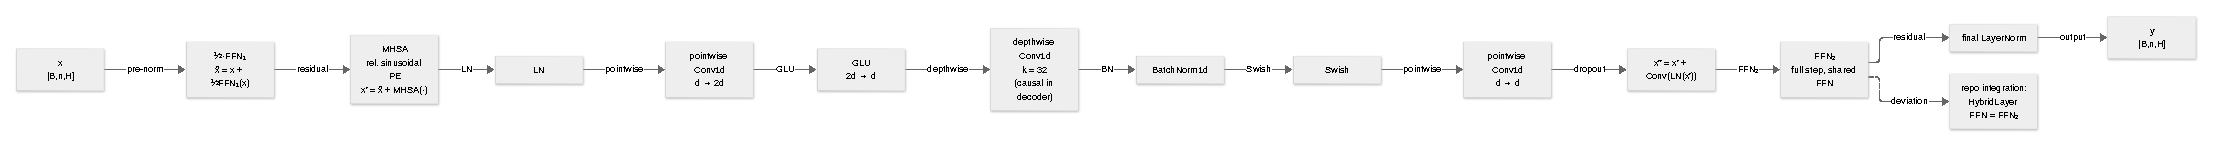
\includegraphics{figures/mixers/conformer.pdf}}
\caption{Dataflow of the Conformer block: a Macaron half-step feed-forward layer, multi-head self-attention with relative sinusoidal positional encodings, the convolution module (pointwise $\to$ GLU $\to$ depthwise $\to$ BatchNorm $\to$ Swish $\to$ pointwise), and the second feed-forward layer followed by the final LayerNorm. In this toolkit the shared \texttt{HybridLayer} feed-forward network plays the $\mathrm{FFN}_2$ slot at a full residual step (dotted annotation).}
\label{fig:mixer-conformer}
\end{figure}

\subsubsection{Mathematical Formulation}

For a block input $x \in \mathbb{R}^{B \times n \times d}$ the reference block of Fig.~1 of \citet{Gulati2020} is
\begin{align}
\tilde{x} &= x + \tfrac{1}{2}\,\mathrm{FFN}_1\big(\mathrm{LN}(x)\big), \label{eq:conformer-ffn1}\\
x' &= \tilde{x} + \mathrm{MHSA}\big(\mathrm{LN}(\tilde{x})\big), \label{eq:conformer-mhsa}\\
x'' &= x' + \mathrm{Conv}\big(\mathrm{LN}(x')\big), \label{eq:conformer-conv}\\
y &= \mathrm{LN}\Big(x'' + \tfrac{1}{2}\,\mathrm{FFN}_2\big(x''\big)\Big). \label{eq:conformer-ffn2}
\end{align}
The two feed-forward terms carry the Macaron \emph{half-step} coefficient: each contributes half of a full residual update, one before and one after the attention--convolution pair.

\paragraph{Feed-forward module.} With hidden width $d_{ff}$,
\begin{equation}
\mathrm{FFN}(x) = W_2\,\mathrm{Dropout}\big(\mathrm{Swish}(W_1\,\mathrm{LN}(x) + b_1)\big) + b_2,
\qquad
\mathrm{Swish}(a) = a\,\sigma(a),
\label{eq:conformer-ffn}
\end{equation}
where $W_1 \in \mathbb{R}^{d_{ff} \times d}$, $W_2 \in \mathbb{R}^{d \times d_{ff}}$ and $\sigma$ is the logistic sigmoid. The paper uses $d_{ff} = 4d$.

\paragraph{Multi-head self-attention with relative positional encoding.} Queries, keys and values are linear projections of the normalized block input, $Q = \mathrm{LN}(\tilde{x})W_Q$, $K = \mathrm{LN}(\tilde{x})W_K$, $V = \mathrm{LN}(\tilde{x})W_V$, split into $H$ heads of width $d_h = d/H$. Following the Transformer-XL relative scheme \citep{Dai2019}, the score of query $i$ against key $j$ adds a sinusoidal function of the \emph{displacement} $i-j$ instead of an absolute position:
\begin{equation}
e_{ij} = q_i^{\top} k_j + (q_i + v)^{\top} R_{i-j},
\qquad
A_{ij} = \operatorname{softmax}_j\!\Big(\frac{e_{ij}}{\sqrt{d_h}}\Big),
\qquad
O = A V W_O,
\label{eq:conformer-relpe}
\end{equation}
with $v$ a learned bias vector and, for $m = 0, \dots, d_h/2 - 1$,
\begin{equation}
R_{\delta,\,2m} = \sin\!\big(\delta\,/\,10000^{2m/d_h}\big),
\qquad
R_{\delta,\,2m+1} = \cos\!\big(\delta\,/\,10000^{2m/d_h}\big).
\label{eq:conformer-sinusoid}
\end{equation}
Because the encoding depends only on $\delta = i-j$, the block generalizes across utterance lengths. The toolkit routes positional information through the model-wide machinery that every other mixer uses: \texttt{model.positional\_encoding} (RoPE by default) is applied to $Q/K$, and \texttt{conformer\_use\_pe} (default \texttt{true}) lets a layer opt out. The paper's relative sinusoidal scheme is closest to \texttt{sinusoidal\_rotary} (sinusoidal frequencies applied as a rotation on $Q/K$, relative by construction); \texttt{alibi}/\texttt{bam} supply a distance bias instead of a rotation. A dedicated Transformer-XL-style relative-sinusoidal module is not implemented. In decoder mode the score matrix receives the usual causal mask before the softmax, and the fixed-softmax path of Appendix~\ref{sec:fixed-implementation} is used when \texttt{numerics.fixed\_softmax} is enabled.

\paragraph{Convolution module.} The module applies a gated depthwise convolution over the time axis:
\begin{align}
h &= \mathrm{LN}(x'), \\
[u,\, g] &= \mathrm{Conv1d}_{d \to 2d}(h), \qquad
\tilde{h} = u \odot \sigma(g), \label{eq:conformer-glu}\\
z_t &= \sum_{k=0}^{K-1} w_k\, \tilde{h}_{t + k - \lfloor K/2 \rfloor}, \label{eq:conformer-depthwise}\\
c &= \mathrm{Dropout}\Big(\mathrm{Conv1d}_{d \to d}\big(\mathrm{Swish}(\mathrm{BN}(z))\big)\Big), \label{eq:conformer-conv-out}
\end{align}
where $\odot$ is the elementwise product (a GLU that halves the $2d$ channels back to $d$), $w \in \mathbb{R}^{K}$ is the depthwise kernel and $\mathrm{BN}$ normalizes each channel over the batch and time axes,
\begin{equation}
\mathrm{BN}(z)_{b,t,c} = \gamma_c\,\frac{z_{b,t,c} - \mu_c}{\sqrt{\sigma_c^2 + \epsilon}} + \beta_c .
\label{eq:conformer-bn}
\end{equation}
In decoder mode the sum in Equation~\ref{eq:conformer-depthwise} is shifted to $z_t = \sum_{k=0}^{K-1} w_k \tilde{h}_{t-K+1+k}$, so that no future frame enters the convolution; encoder and ViT modes keep the symmetric ``same'' padding of the paper.

\subsubsection{Algorithmic Pseudocode}

\begin{algorithm}[H]
\caption{Conformer block (\texttt{conformer})}
\begin{algorithmic}[1]
\Require block input $x \in \mathbb{R}^{B \times n \times d}$, kernel $K=32$, heads $H$, Macaron flag, mode
\Ensure block-level delta $\Delta$ such that $x + \Delta$ enters the outer $\mathrm{norm}_2 + \mathrm{FFN}_2$
\State $\tilde{x} \gets x + \mathrm{FFN}_1(\mathrm{LN}(x))$ \Comment{Macaron FFN$_1$ ($\tfrac12$ in the paper)}
\State $Q, K_{proj}, V \gets \mathrm{LN}(\tilde{x})W_Q,\ \mathrm{LN}(\tilde{x})W_K,\ \mathrm{LN}(\tilde{x})W_V$
\State $e_{ij} \gets q_i^{\top}k_j + (q_i + v)^{\top}R_{i-j}$ \Comment{relative sinusoidal PE, Eq.~\ref{eq:conformer-relpe}}
\If{mode $=$ decoder}
    \State $e_{ij} \gets -\infty$ for $j > i$ \Comment{causal mask}
\EndIf
\State $x' \gets \tilde{x} + \mathrm{softmax}(e/\sqrt{d_h})\,V\,W_O$
\State $h \gets \mathrm{LN}(x')$
\State $[u, g] \gets \mathrm{Conv1d}_{d \to 2d}(h)$; \quad $\tilde{h} \gets u \odot \sigma(g)$ \Comment{GLU}
\State $z \gets \mathrm{DepthwiseConv1d}_{K}(\tilde{h})$ \Comment{causal shift in decoder mode}
\State $c \gets \mathrm{Dropout}(\mathrm{Conv1d}_{d \to d}(\mathrm{Swish}(\mathrm{BN}(z))))$
\State $x'' \gets x' + c$
\State \Return $x''$ \Comment{\texttt{HybridLayer} adds $\mathrm{FFN}_2$ and the final LN}
\end{algorithmic}
\end{algorithm}

\subsubsection{Implementation Mapping and Deviations}

Table~\ref{tab:conformer-mapping} maps the paper block onto the toolkit. The substantive deviations are the two residual scalings and the second feed-forward layer: the paper keeps both $\tfrac12$ Macaron coefficients and wraps $\mathrm{FFN}_2$ in the block, whereas \texttt{conformer} uses full steps and returns the state after the convolution module, letting the outer \texttt{HybridLayer} apply its shared $\mathrm{norm}_2 + \mathrm{FFN}$ (also at full step). The decomposition is deliberate---it keeps MoE routing, Mixture-of-Depths, mHC/Hyperloop streams, AttnRes, FlashNorm fusion, BitNet projections and the per-parameter-group optimizer routing available for the second FFN, none of which would survive a private FFN inside the mixer.

\begin{table}[H]
\centering
\small
\begin{tabularx}{0.95\linewidth}{L{3.6cm}L{4.4cm}X}
\toprule
\textbf{Paper component} & \textbf{Toolkit implementation} & \textbf{Notes} \\
\midrule
$\tfrac{1}{2}\mathrm{FFN}_1$ (pre-norm) & private FFN inside \texttt{ConformerAttention}; Swish; full-step residual & \texttt{conformer.macaron: true} (default); the $\tfrac12$ coefficient of the paper is dropped; disabling leaves attention $+$ convolution only \\
MHSA, relative sinusoidal PE & own $q/k/v/out$ projections; model-wide PE via \texttt{conformer\_use\_pe} (default \texttt{true}) & paper's relative sinusoid $\approx$ \texttt{sinusoidal\_rotary}; no dedicated Transformer-XL module (RoPE is the model-wide default) \\
Convolution module & LN $\to$ pointwise $\to$ GLU $\to$ depthwise $\to$ BN $\to$ Swish $\to$ pointwise $\to$ dropout & \texttt{conformer.kernel\_size} (32), \texttt{conformer.conv\_norm} (\texttt{batch}/\texttt{group}/\texttt{layer}) \\
$\tfrac{1}{2}\mathrm{FFN}_2$ at half step & \texttt{HybridLayer} $\mathrm{norm}_2 + \mathrm{FFN}$, full step & justified by Table~5 of \citet{Gulati2020}: $1.9/4.4$ vs.\ $1.9/4.5$ dev WER (both coefficients dropped) \\
Final LayerNorm & \texttt{HybridLayer} final norm & unchanged from every other mixer \\
4$\times$ convolutional subsampling & \texttt{frankenstein\_audio} frontend & Appendix~\ref{sec:annex-audio}; text/ViT use their own embeddings \\
Dropout ($p=0.1$) & \texttt{model.dims.dropout} & global, per-block \\
\bottomrule
\end{tabularx}
\caption{Implementation mapping of the Conformer block. The deviations are the dropped $\tfrac12$ Macaron scalings, the second FFN (supplied by the outer layer at full step) and the positional-encoding plumbing.}
\label{tab:conformer-mapping}
\end{table}

\paragraph{Why the full-step FFN is safe.} Dropping the Macaron $\tfrac12$ changes the per-branch residual scale, not the expressive form of the block: the full-step variant is exactly what \citet{Gulati2020} ablate in their Table~5, where it moves dev-clean/dev-other WER from $1.9/4.4$ (half step) to $1.9/4.5$ (full step), i.e.\ one tenth of a point. The toolkit therefore uses full steps for both feed-forward layers; the first stays private to the mixer, and the second is the shared one, which preserves the composability described above.

\subsection{Published Ablations}

Table~\ref{tab:conformer-ablations} summarizes the ablations that motivate the default configuration. Values are the ones reported by \citet{Gulati2020}; the qualitative ordering is what the defaults encode.

\begin{table}[H]
\centering
\small
\begin{tabularx}{0.95\linewidth}{L{3.7cm}L{4.0cm}X}
\toprule
\textbf{Ablation} & \textbf{Settings compared} & \textbf{Reported outcome} \\
\midrule
Convolution module (Table~3) & present vs.\ removed & the largest single degradation of the block when removed; the local branch is load-bearing, not decorative \\
Macaron FFN pair (Table~3) & $\tfrac{1}{2}\mathrm{FFN}_1 + \tfrac{1}{2}\mathrm{FFN}_2$ vs.\ one FFN & removing the pair costs roughly $0.2$ dev-clean / $0.5$ dev-other WER \\
Half vs.\ full step (Table~5) & $\tfrac{1}{2}$ residuals vs.\ full residuals & $1.9/4.4$ vs.\ $1.9/4.5$ dev WER: at most $0.1$ point \\
Kernel size (Table~7) & $K \in \{3, 7, 17, 32, 65\}$ & $K = 32$ is best; small kernels under-fit the local context, $K = 65$ adds cost without gain \\
Conv placement & after MHSA, before $\mathrm{FFN}_2$ & reference order retained; moving the branch does not improve on it \\
\bottomrule
\end{tabularx}
\caption{Conformer ablations and the defaults they justify (\texttt{kernel\_size: 32}, \texttt{macaron: true}, full-step shared $\mathrm{FFN}_2$).}
\label{tab:conformer-ablations}
\end{table}

\subsection{Reuse of Existing Infrastructure}

Because \texttt{ConformerAttention} returns a delta and inherits the \texttt{mixer(config, pos\_encoder=...)} constructor, the entire stack is reused without special cases:

\begin{itemize}[leftmargin=*]
    \item \textbf{Model classes:} text encoder (\texttt{mlm}/\texttt{sbert}/\texttt{text\_classification}), causal decoder (\texttt{causal\_lm}), Vision Transformer (\texttt{patch\_prediction}/\texttt{classification}/\texttt{segmentation}) and \texttt{frankenstein\_audio} (\texttt{asr}, \texttt{audio\_classification}).
    \item \textbf{Normalization:} all 6 variants, including partial RMSNorm and FlashNorm fusion on $\mathrm{norm}_1$/$\mathrm{norm}_2$; the convolution module keeps its own BatchNorm unless \texttt{conformer.conv\_norm} selects group or layer normalization.
    \item \textbf{Routing and residuals:} MoE, Mixture-of-Depths, mHC, Hyperloop, AttnRes and the BitNet ternary projections (the private FFN and the convolution projections are BitLinear-aware).
    \item \textbf{Optimizers:} all 23 families with per-group prefixes; mixer parameters, including the depthwise kernel and the convolution norms, route to the \texttt{attention} group.
    \item \textbf{KV cache:} \texttt{conformer} is registered as \emph{not} cacheable (\texttt{supported=False}), because the depthwise-convolution state and the BatchNorm running statistics would have to be carried across steps. \texttt{generate()} falls back to the full-recompute path, which is exact.
\end{itemize}

\subsection{When to Use It}

\begin{itemize}[leftmargin=*]
    \item \textbf{Speech:} the default mixer for \texttt{asr} and \texttt{audio\_classification}; at 40\,ms frames after $4\times$ subsampling the kernel of 32 spans $\sim$1.28\,s of context, roughly the width of a phone sequence.
    \item \textbf{Text and vision:} a strong drop-in for \texttt{standard} when the data has local structure (character-level models, code, OCR, patch sequences); it costs one depthwise convolution and two extra norms per layer over a plain attention block.
    \item \textbf{Streaming decoding:} usable in \texttt{mode: decoder} with causal convolution padding, but without the incremental cache of Appendix~\ref{sec:annex-kv-cache}; the depthwise recurrence is the missing piece.
\end{itemize}

\subsection{Fast Conformer: Limited-Context Attention with a Head-Pinned Global Token}

\begin{figure}[H]
\centering
\fitfigure{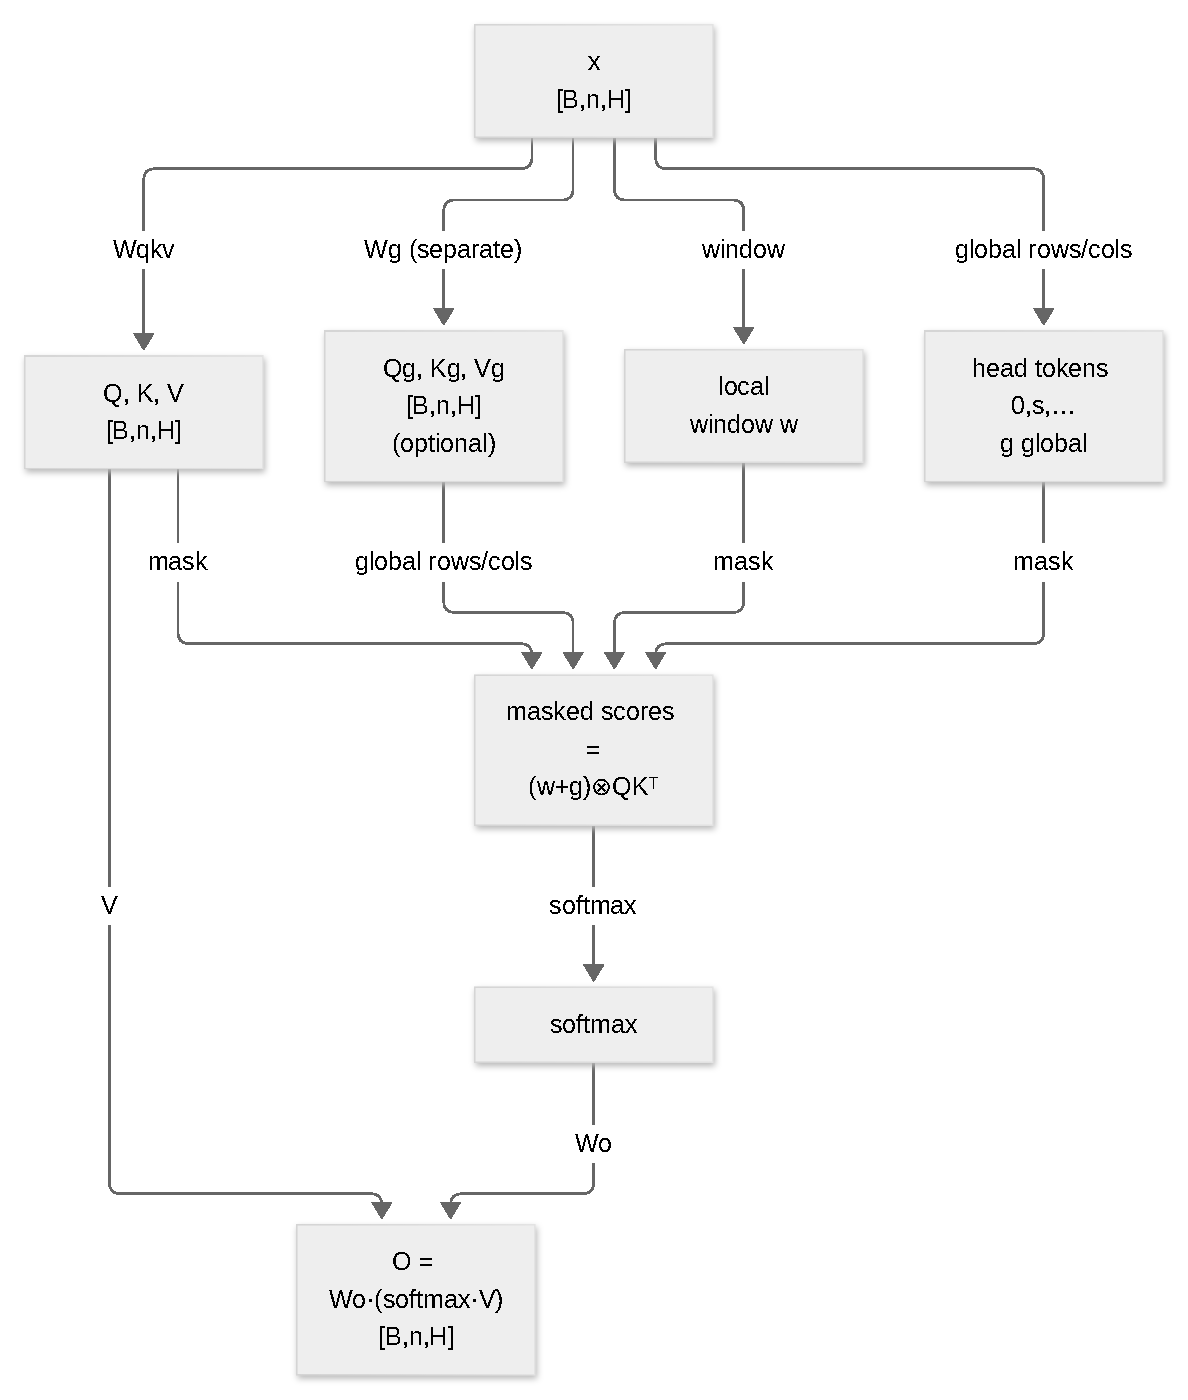
\includegraphics{figures/mixers/fastconformer.pdf}}
\caption{Dataflow of Fast Conformer limited-context attention: every query attends to a symmetric local window, while a small set of global attention tokens pinned at the head of the sequence attend to every position and are attended by every position; the global token may use its own query/key/value projections (paper \S2.2).}
\label{fig:mixer-fastconformer}
\end{figure}

\subsubsection{Mathematical Formulation}

Fast Conformer \citep{rekesh_fastconformer_2023} attacks the quadratic cost of Conformer self-attention in two ways: it raises the front-end downsampling to $8\times$, and, for long-form inputs, it replaces global attention with \emph{limited-context} attention. The paper describes the mixer in prose rather than in display equations: ``we use a single global attention token, which attends to all other tokens and has all other tokens attend to it, using a separate set of query, key and value linear projections, while others attend in a fixed-size window surrounding each token'' (\S2.2), while the evaluated long-form model ``has shared query, key and value projection layers that are used for global and local attention'' (\S3.4) and sets ``the size of the limited context \ldots to 128 steps on each side of a token''. This implementation encodes exactly that description and inherits the global-attention dataflow from Longformer \citep{beltagy_longformer_2020}, which the paper explicitly cites for the mechanism and for its overlapping-chunk kernel.

Let $X \in \mathbb{R}^{n \times H}$ be the layer input, $h$ the number of heads and $d = H/h$. The shared projections are
\[
\mathbf{Q} = X\mathbf{W}_Q, \qquad \mathbf{K} = X\mathbf{W}_K, \qquad \mathbf{V} = X\mathbf{W}_V,
\]
with $\mathbf{W}_\ast \in \mathbb{R}^{H \times H}$ and no bias. The optional global projections of the paper's \S2.2 variant are a second set,
\[
\mathbf{Q}^{g} = X\mathbf{W}_Q^{g}, \qquad \mathbf{K}^{g} = X\mathbf{W}_K^{g}, \qquad \mathbf{V}^{g} = X\mathbf{W}_V^{g},
\]
which adds $3H^2$ parameters; the \S3.4 evaluated model sets $\mathbf{W}_\ast^{g} = \mathbf{W}_\ast$.

The global positions are the head of the sequence, spaced $s$ apart,
\[
\mathcal{G} = \{\,0, s, 2s, \dots, (g-1)s\,\},
\]
so a global token is a designated input position rather than an extra learned embedding (the paper's ``addition of a global token''). The attention pattern is
\[
M_{ij} = \big[\,|i-j| \le w/2\,\big] \;\vee\; \big[\,j \in \mathcal{G}\,\big] \;\vee\; \big[\,i \in \mathcal{G}\,\big],
\]
where the first term is the local window, the second lets every query attend to the global tokens, and the third lets a global token attend to every position; $M$ is intersected with the causal mask in decoder mode. With the effective keys and values
\[
\tilde{\mathbf{k}}_j = \begin{cases} \mathbf{k}^{g}_j & j \in \mathcal{G}\ \text{and separate}, \\ \mathbf{k}_j & \text{otherwise}, \end{cases}
\qquad
\tilde{\mathbf{v}}_j = \begin{cases} \mathbf{v}^{g}_j & j \in \mathcal{G}\ \text{and separate}, \\ \mathbf{v}_j & \text{otherwise}, \end{cases}
\]
the output is standard scaled dot-product attention over the allowed pairs,
\[
z_{ij} = \frac{\mathbf{q}_i \cdot \tilde{\mathbf{k}}_j}{\sqrt{d}}, \qquad
\mathbf{o}_i = \sum_{j:\,M_{ij}} \operatorname{softmax}_j(z_{ij})\,\tilde{\mathbf{v}}_j, \qquad
\mathbf{Y} = \mathbf{O}\mathbf{W}_O .
\]
In the separate variant a global query row is computed with the global projections over the whole causal prefix, $\mathbf{o}_i = \sum_{j \le i} \operatorname{softmax}_j(\mathbf{q}^{g}_i \cdot \mathbf{k}^{g}_j/\sqrt{d})\,\mathbf{v}^{g}_j$, matching Longformer's global-attention design. With shared projections all three cases collapse to one $\mathbf{Q}/\mathbf{K}/\mathbf{V}$ set: the global tokens are simply positions with unmasked rows and columns.

\subsubsection{Algorithmic Pseudocode}

\begin{algorithm}[H]
\caption{Fast Conformer limited-context attention (masked-dense reference form)}
\begin{algorithmic}[1]
\Require Input $X$; window $w$; global count $g$; spacing $s$; separate flag
\Ensure Output $\mathbf{Y}$
\State $\mathbf{Q},\mathbf{K},\mathbf{V} \gets X\mathbf{W}_Q, X\mathbf{W}_K, X\mathbf{W}_V$
\If{separate}
    \State $\mathbf{Q}^{g},\mathbf{K}^{g},\mathbf{V}^{g} \gets X\mathbf{W}_Q^{g}, X\mathbf{W}_K^{g}, X\mathbf{W}_V^{g}$
    \State $\tilde{\mathbf{K}}, \tilde{\mathbf{V}} \gets \mathbf{K}, \mathbf{V}$; replace rows $\mathcal{G}$ with $\mathbf{K}^{g}, \mathbf{V}^{g}$
\Else
    \State $\tilde{\mathbf{K}}, \tilde{\mathbf{V}} \gets \mathbf{K}, \mathbf{V}$
\EndIf
\State $\mathcal{G} \gets \{0, s, \dots, (g-1)s\}$ clipped to $n$
\State $M \gets [\,|i-j| \le w/2\,] \vee [\,j \in \mathcal{G}\,] \vee [\,i \in \mathcal{G}\,]$
\If{decoder} $M \gets M \wedge [\,j \le i\,]$ \EndIf
\State $Z \gets \mathbf{Q}\tilde{\mathbf{K}}^{\top}/\sqrt{d}$ masked by $M$
\If{separate \textbf{and} $\mathcal{G} \ne \emptyset$}
    \State $Z[\mathcal{G},:] \gets \mathbf{Q}^{g}[\mathcal{G}]\mathbf{K}^{g\top}/\sqrt{d}$ (causal-clipped)
\EndIf
\State $\mathbf{O} \gets \operatorname{softmax}(Z)\tilde{\mathbf{V}}$
\If{separate \textbf{and} $\mathcal{G} \ne \emptyset$}
    \State $\mathbf{O}[\mathcal{G},:] \gets \operatorname{softmax}(Z[\mathcal{G},:])\mathbf{V}^{g}$ \Comment{global rows aggregate global values}
\EndIf
\State $\mathbf{Y} \gets \mathbf{O}\mathbf{W}_O$
\end{algorithmic}
\end{algorithm}

In incremental decoding the retained state is a bounded ring: the pinned head region covers $\mathcal{G}$ and the ring keeps the last $w/2+1$ keys, so each step costs $\mathcal{O}(w+g)$. The exact pattern is evaluated against the cached absolute positions (unlike a retention-equals-pattern shortcut, because a spaced global prefix may contain non-global positions).

\subsubsection{Key Characteristics}

\begin{itemize}[leftmargin=*]
    \item \textbf{Complexity}: $\mathcal{O}(n\,(w+g)\,d)$ training and $\mathcal{O}(w+g)$ per decoded token with the paper's overlapping-chunk kernel; the reference implementation here masks a dense score matrix, which is mathematically identical but $\mathcal{O}(n^2)$ in compute. Memory is bounded by $w+g$.
    \item \textbf{Trainable}: Yes, natively from scratch (the pattern runs in both training and evaluation). The paper fineTunes a full-context checkpoint for 10k steps at peak LR $10^{-6}$ with a 1k-step warmup and cosine decay, but the mixer's weights are ordinary attention projections.
    \item \textbf{Strength}: On long-form benchmarks the global token is the decisive ingredient: normalized greedy WER improves from 9.18 (Conformer) to 8.25 (limited context) to \textbf{7.5} (plus global token) on TED-LIUM v3, and from 18.26 to 16.08 to \textbf{11.85} on Earnings-21, while the single-pass maximum duration grows from 15 to 675 minutes on one A100. The encoder is $2.8\times$ faster and uses $2.9\times$ fewer multiply-accumulates than the original Conformer.
    \item \textbf{Limitation}: The paper gives no closed-form equations for the global-token path (the formulation above is a documented reconstruction from its prose, Longformer and the authors' NeMo recipe). The default is a single global token with shared projections; the separate-projection variant costs $3H^2$ extra parameters and is only exact in the cached path when the global queries are pre-filled from position zero. The efficient chunked kernel is not implemented.
\end{itemize}
